\documentclass{report}
\usepackage{comment}
\usepackage{fancyhdr}
\pagestyle{fancy}

\rhead{ \thepage}
\cfoot{  }
\rfoot{Suryanshu, 22BCE0820}
\renewcommand{\headrulewidth}{0.4pt}
\renewcommand{\footrulewidth}{0.4pt}
\usepackage{listings}
\title{\textbf{Finlatics \\ Programme: Business Analytics \\ Project 2}}

\author{Suryanshu}
\usepackage{titlesec}
\titleformat
{\chapter} % command
[display] % shape
{\bfseries\Large\itshape} % format
{Business Analytics} % label
{0.5ex} % sep
{
    \rule{\textwidth}{1pt}
    \vspace{1ex}
    \centering
} % before-code
[
\vspace{-0.5ex}%
\rule{\textwidth}{0.3pt}
] % after-code

\usepackage{tikz}
\usetikzlibrary{shapes.geometric, arrows}

\tikzstyle{startstop} = [rectangle, rounded corners, minimum width=3cm, minimum height=1cm,text centered, draw=black, fill=red!30]

%\tikzstyle{process} = [rectangle, minimum width=3cm, minimum height=1cm, text centered, draw=black, fill=orange!30]

\tikzstyle{io} = [trapezium, trapezium left angle=70, trapezium right angle=110, minimum width=1cm, minimum height=1cm, text centered, text width=1.5cm, draw=black, fill=blue!30]

\tikzstyle{layer2} = [rectangle, minimum width=2cm, inner sep=7pt, text centered,  draw=black, fill=orange!30]
\tikzstyle{layer3} = [rectangle, text centered, text width=2.5cm, inner sep=7pt, draw=black, fill=blue!30]
\tikzstyle{layer4} = [rectangle, text centered, text width=2.5cm, inner sep=7pt, draw=black, fill=green!30]

\tikzstyle{decision} = [diamond, minimum width=3cm, minimum height=1cm, text centered, draw=black, fill=green!30]
\tikzstyle{line} = [draw, -latex']
\tikzstyle{arrow} = [thick,->,>=stealth]
\begin{document}
\maketitle
\tableofcontents

\chapter{Project 2 }
\section{Introduction}
The problem statement requires us to do two basic things:
\begin{enumerate}
  \item \textbf{Data Processing:} Convert the unstructured-map data, into structured data-excel sheet. And from this find various information regarding the data set like:
  \begin{itemize}
    \item State with the hightest number of hotels
    \item Filtering out the states with three types of climates
    \item Average number of days the rainy season lasts in Indian states
  \end{itemize}
\item \textbf{Analytics:} After processing the data, it must be interpretted and analysed. From this analysis we must suggest:
  \begin{itemize}
    \item Among the northeastern states which are best to set up a hotel
    \item Which is the best state for setting up a hotel
  \end{itemize}
\end{enumerate}
\newpage
Here is the map provided.
\begin{Center}
  \begin{figure}[h!]
    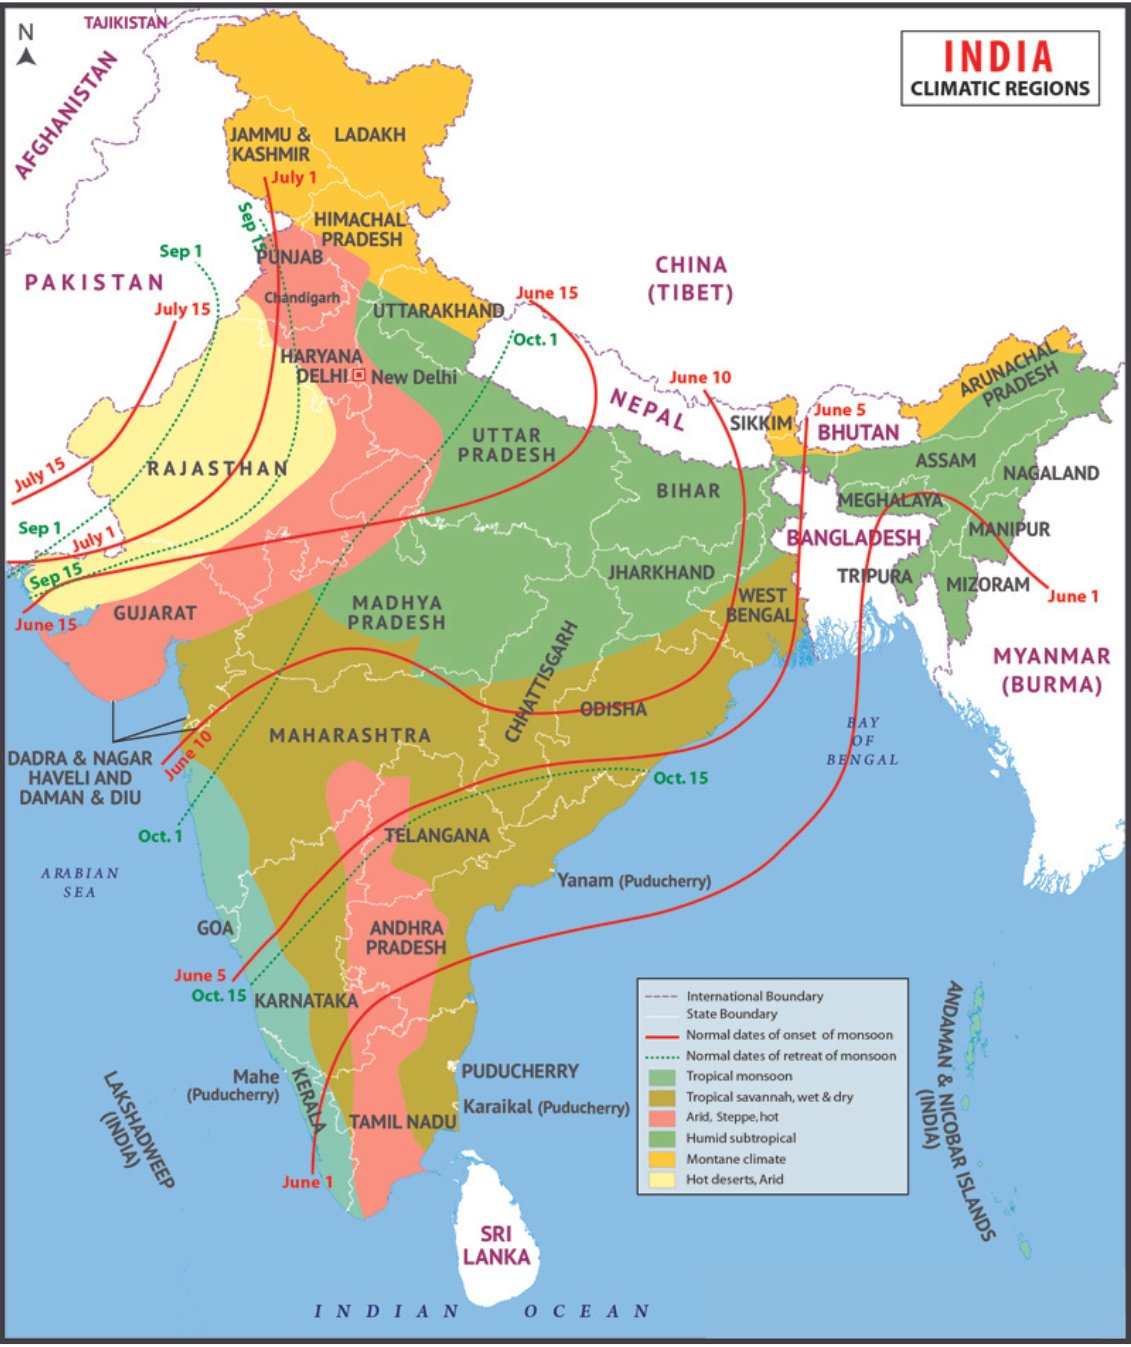
\includegraphics[width=1\textwidth]{map.png}
    \caption{Map of Climatic Regions in India}
   \end{figure}
 \end{Center}
\section{Data Processing}
The first step here is to process the Hotel\_Dataset provided. Then we convert the unstructured-map data into structure-excel sheet(the different climates and the onset and retreat of monsoon in each state).
 \newpage
\subsection{Hotel\_Dataset}
\begin{Center}
  \begin{figure}[h!]
    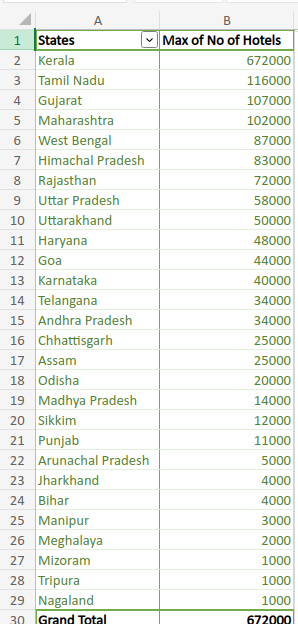
\includegraphics[width=0.6\textwidth]{Hotel_Dataset.png}
    \caption{Hotel Dataset in a sorted pivot table}
   \end{figure}
 \end{Center}
 From this we learn that \textbf{Kerala} has the hightest number of hotels, i.e. 672000.
\newpage
This data can be presented via a bar graph which compares all the states.
\begin{Center}
  \begin{figure}[h!]
    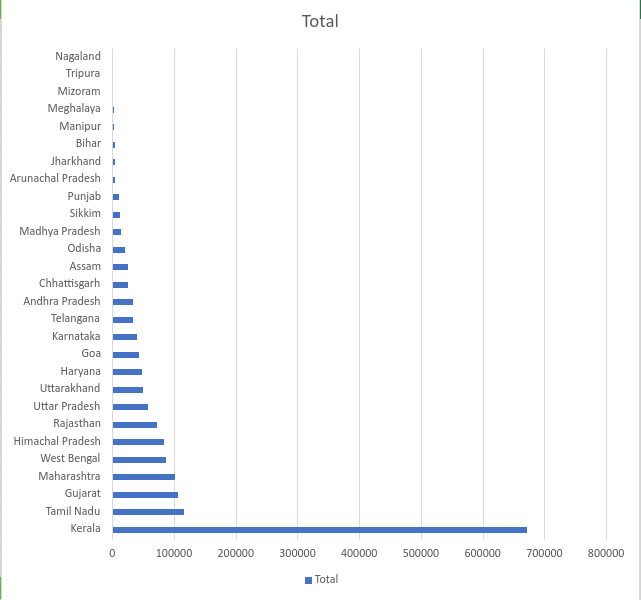
\includegraphics[width=0.85\textwidth]{Hotel_BarGraph.png}
    \caption{Hotel Dataset in a bar graph}
   \end{figure}
\end{Center}
\newpage 
\subsection{Climatic Conditions}
Here we convert the map into two excelsheets- first for the types of climates in a state, second the number of days of rainy season.
\begin{Center}
  \begin{figure}[h!]
    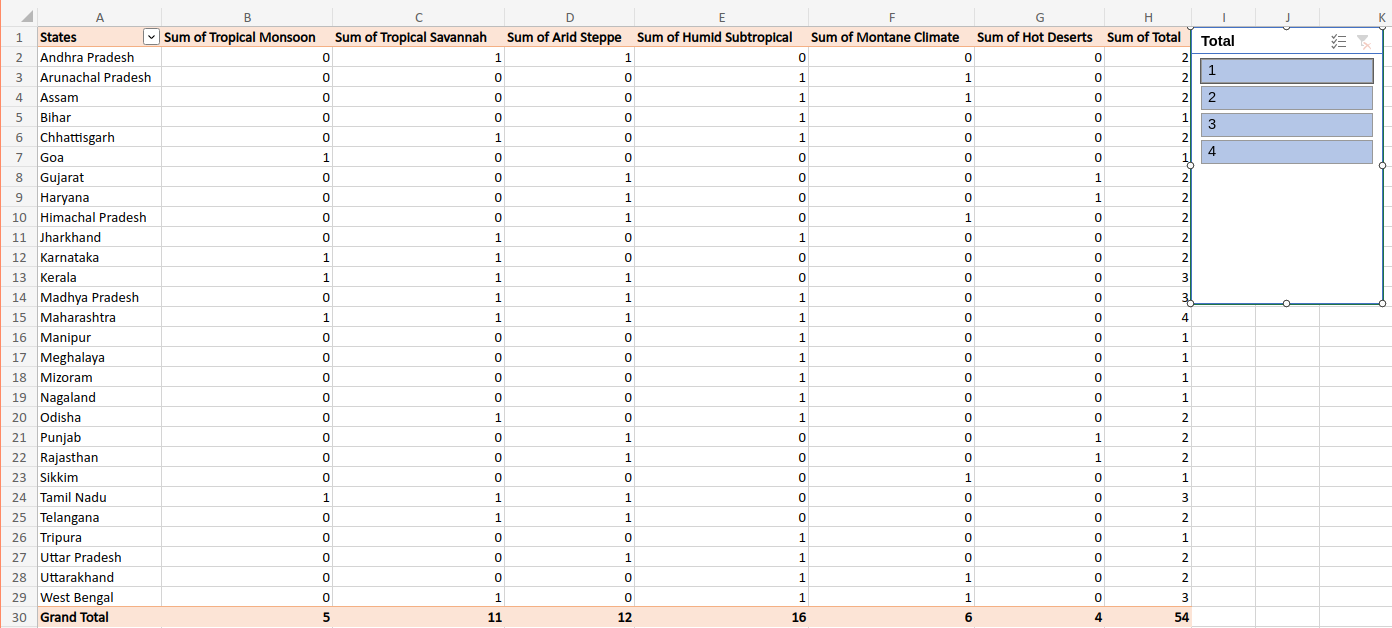
\includegraphics[width=1.25\textwidth]{ClimateData.png}
    \caption{Weather Data into a tabular form}
   \end{figure}
 \end{Center}
\\ From this we filter out the states which have three types of climatic conditions.
\begin{Center}
  \begin{figure}[h!]
    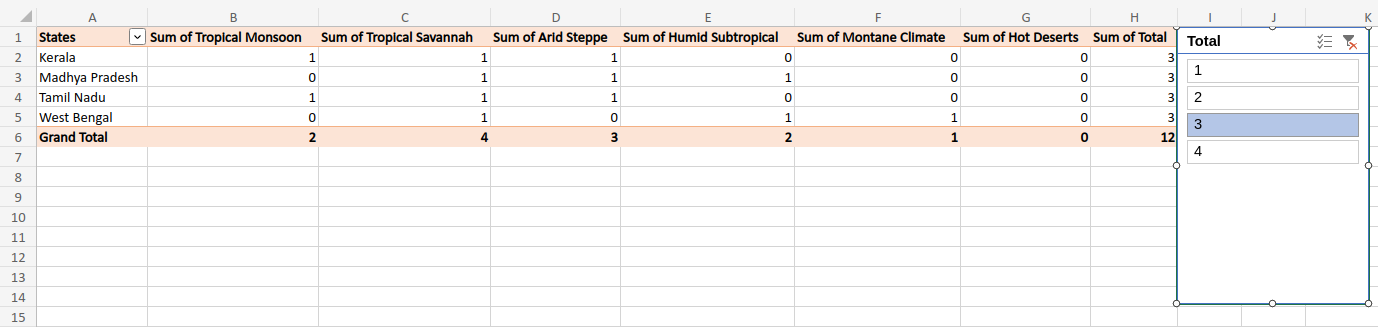
\includegraphics[width=1.25\textwidth]{ClimateDataFiltered.png}
    \caption{Filtered Data}
   \end{figure}
 \end{Center}
 \\
 We find that 4 states namely-
\begin{itemize}
    \item Kerala
    \item Madhya Pradesh
    \item Tamil Nadu
    \item West Bengal
  \end{itemize}
have three types of climatic condtions.
\newpage
Now we follow the datelines presented and convert the monsoon onset and retreat into structured data.
\begin{Center}
  \begin{figure}[h!]
    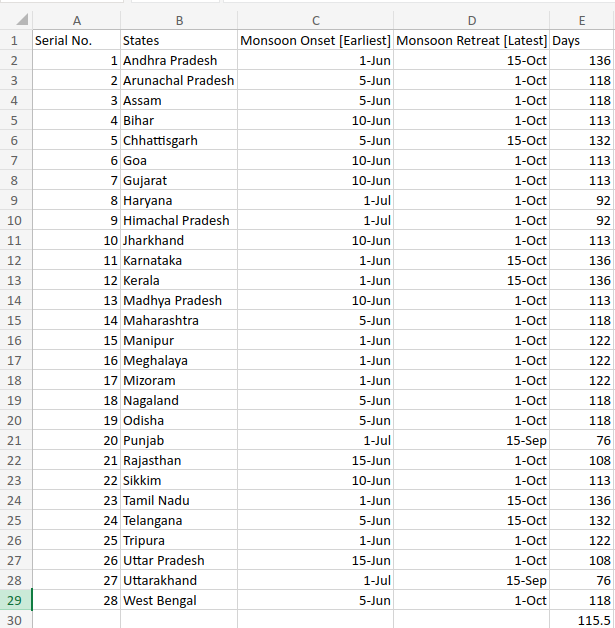
\includegraphics[width=0.85\textwidth]{AvgMonsoon.png}
    \caption{Average number of days the rainy season lasts in Indian states}
   \end{figure}
 \end{Center}
\\ From this we calculate the average number of days the rainy season lasts in Indian states, which comes out to be 115.5 days.
\newpage
\subsection{Data on Northeastern States}
In order to analyse the northeastern states of India, we'll separate their data from the rest and then reprocess it.
\begin{Center}
  \begin{figure}[h!]
    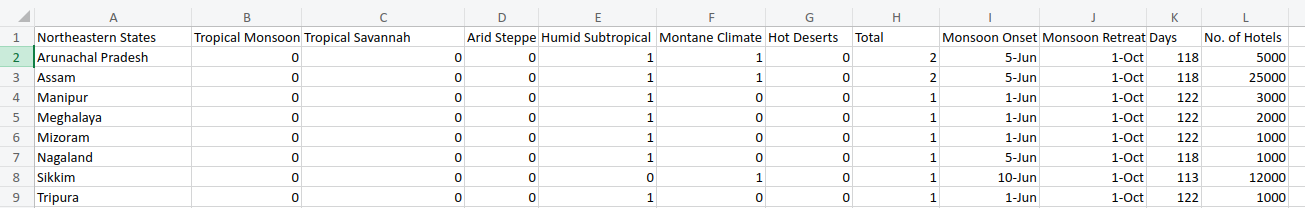
\includegraphics[width=1.35\textwidth]{NEData.png}
    \caption{Northeastern States' Data}
   \end{figure}
 \end{Center}
\\ We make a separate pivot table for the average of days and average number of hotels.
\begin{Center}
  \begin{figure}[h!]
    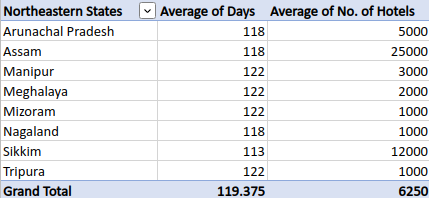
\includegraphics[width=1\textwidth]{NEPivotHotelandMonsoon.png}
    \caption{Hotel and Monsoon NE Pivot Table}
   \end{figure}
 \end{Center}
\newpage
We make a clustered bar graph to compare all the NE states in terms of rainy days and number of hotels
\begin{Center}
  \begin{figure}[h!]
    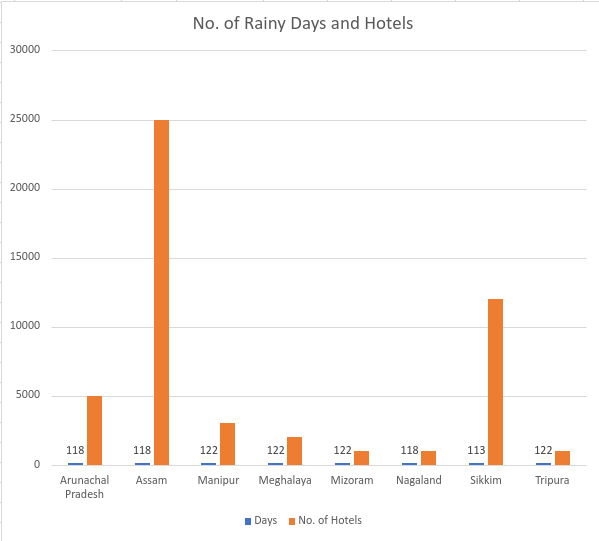
\includegraphics[width=1\textwidth]{NEColumnBar.png}
    \caption{Number of Rainy Days and Hotels in NE states}
   \end{figure}
 \end{Center}
\newpage
 We use a stacked bar graph to identify the proportion of different climatic conditions present in the NE region.
\begin{Center}
  \begin{figure}[h!]
    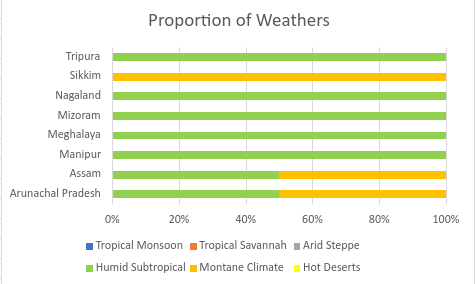
\includegraphics[width=1\textwidth]{NEWeatherBar.png}
    \caption{Proportion of Climatic Conditions in the NE region}
   \end{figure}
 \end{Center}
 \\ This concludes our data processing part and we move on to analysing this data to draw conclusions out of it.
 \section{Analytics}
 We have three factors to analyse whether a state is optimal to set up a hotel or not.
 \begin{itemize}
 \item \textbf{Climatic Condtions:} We pick the state with moderate climate, if the the weather's too harsh, tourists are unlikely to show up.
 \item \textbf{Monsoon:} Tourists would rarely travel in monsoon, hence the state with fews rainy days would be preferred.
 \item \textbf{Number of already established hotels:} If the competition is too hgh that would negatively impact the business.
 \end{itemize}
 \subsection{Best Northeastern state to set up a hotel}

 After analysing the data we find that only Sikkim(12000) and Assam(25000) have a huge number of hotels. Either we can establish hotels in those states and face fierce competition or we can invest in \textbf{Meghalaya}(2000) and \textbf{Arunachal Pradesh}(5000) with moderate competition and hence still an untapped market.
Even weather seems favourable for Arunachal Pradesh and Meghalaya which recieve rains for 118 and 122 days respectively with a humid subtropical climate.
 \subsection{Best state to set up a hotel}
 As a hotel requires a good influx of tourists in order to thrive, we must look at what attracts tourists in the first place. While a tourist attraction is a must, but there must be an already state established infrastructure to support tourism.

 We find that \textbf{Karnataka} with all its natural beauty, tourist and religious spots still has on average fewer hotels (hence less competition) than say, Kerala or Tamil nadu. The weather is a mix of wet and dry with tropical monsoon and savannah with it rainy 136 days.
\end{document}
